%%%%%%%%%%%%%%%%%%%%%%%%%%%%%%%%%%%%%%%%%%%%%%%%%%%
%
%  New template code for TAMU Theses and Dissertations starting Fall 2012.  
%  For more info about this template or the 
%  TAMU LaTeX User's Group, see http://www.howdy.me/.
%
%  Author: Wendy Lynn Turner 
%	 Version 1.0 
%  Last updated 8/5/2012
%
%%%%%%%%%%%%%%%%%%%%%%%%%%%%%%%%%%%%%%%%%%%%%%%%%%%

%%%%%%%%%%%%%%%%%%%%%%%%%%%%%%%%%%%%%%%%%%%%%%%%%%%%%%%%%%%%%%%%%%%%%%
%%                           SECTION I
%%%%%%%%%%%%%%%%%%%%%%%%%%%%%%%%%%%%%%%%%%%%%%%%%%%%%%%%%%%%%%%%%%%%%

\pagestyle{plain} % No headers, just page numbers
\pagenumbering{arabic} % Arabic numerals
\setcounter{page}{1}

\chapter{\uppercase {Introduction:}}
Hyperbolic systems of equations are encountered in various engineering fields (extraction of oil, turbine technology, nuclear reactors, etc $\ldots$). Improving numerical solution techniques for such equations is an ongoing topic of research. This is obviously the case for fluid equations. Being able to accurately solve and predict the behavior of a fluid in a turbine or in a reactor, for example, may lead to a safe decrease in conservative safety margins, which translates into a decrease in production cost. Thus, we can see the importance of having a good understanding of the mathematical theory behind these wave-dominated systems of equations and also the importance of developing robust and accurate numerical methods.


A large number of theoretical studies has shown the role played by characteristic equations and the corresponding eigenvalues on how and at what speed the physical information propagates: physical shocks or discontinuities can form, leading to unphysical instabilities and oscillations that pollute the numerical solution due to entropy production \cite{Toro}. Naturally, the following question arises: how to accurately detect and resolve shocks as well as conserve the physical solution at the same time? Numerous works are available in the literature and include Riemann solvers, Godunov-type fluxes, flux limiters, and artificial viscosity methods. Toro's book \cite{Toro} provides a good overview of the theory related to hyperbolic systems of equations and focuses on Riemann solvers and Godunov-type fluxes that can be used with discontinuous spatial discretizations: finite volume (FV) and discontinuous Galerkin finite element method (DGFEM).
Flux limiters \cite{FluxLimiter1, FluxLimiter3} can achieve high-order accuracy with DGFEM \cite{FluxLimiter2} but suffer from some drawbacks: difficulties were found to reach steady-state solutions when using time-stepping schemes and generalization to unstructured grids is not obvious \cite{FluxLimiter4}. The artificial viscosity method was first introduced by Neumann and Richtmeyer \cite{Neumann} but was found to be over-dissipative and, thus, abandoned. Only later, with the development of high-order schemes, that artifical viscosity methods have regained interest: Lapidus \cite{Lapidus_paper, Lapidus_book} developed a high-order viscosity method by making the viscosity coefficient proportional to the gradient of the velocity in 1-D. Lohner et al. \cite{LMP} extended this concept to multi-dimensions by introducing a vector that will measure the direction of maximum change in the absolute value of the velocity norm so that shear layers are not smeared. Pressure-based viscosities were also studied \cite{PBV_book} where the viscosity coefficient is set proportional to the Laplacian of pressure, allowing the detection of curvature changes in the pressure profile. Since pressure is often nearly constant except in shock regions, the Laplacian of pressure is a good indicator of the presence of a shock.
Recently, Reisner et al. \cite{Reisner} introduced the C-method for the compressible Euler equations with artificial dissipative terms: instead of computing the viscosity coefficient on the fly as for Lapidus' and pressure-based methods, a partial differential equation (PDE) is added to the original system of equations. This additional PDE is solved for the viscosity coefficient and contains a source term that is function of the gradient of velocity. Numerical results presented using the C-method indicate it yields satisfactory results in 1-D for a wide range of test cases. 
Guermond et .al \cite{jlg1, jlg2, jlg3} proposed an entropy-based viscosity method for conservative hyperbolic system of equations. In their technique, artificial dissipative terms are added to the system of equations with a viscosity coefficient modulated by the entropy production that is known to be large in shocks and small everywhere else. The method was successfully applied using various spatial discretizations \cite{jlg2, jlg3, valentin} and showed high-order convergence with smooth solutions. Results using the ideal gas equation of state were run for 1-D Sod tube and showed good agreement with the exact solutions. 2-D tests were also performed on unstructured grids and behaved very satisfactorily \cite{jlg1,valentin}. The method is fairly simple to implement and is consistent with the entropy minimum principle.


The objective of this Dissertation is to solve hyperbolic system of equations using a \emph{continuous} Galerkin finite element method (CGFEM) with an implicit temporal discretization within the MOOSE framework \cite{Moose}. We are particularly interested in simulating flow behaviors occurring in nuclear reactors. The set of equations that will be considered are the multi-D Euler equations with variable area \cite{Toro} and the multi-D seven-equations model for two-phase fluids \cite{SEM}. These systems of equations are hyperbolic and well defined in a sense that they possess real eigenvalues. To numerically solve these equations, we need to rely on a numerical method that can resolve shocks and discontinuities that may form. Furthermore, we need a method that is accurate for a wide range of Mach numbers and is not restricted to any type of equation of state. These requirements may be hard to fulfill. Numerical methods are often tested with the ideal gas equation of state which can not be used for liquid phase. Another difficulty deals with devising a numerical method that is valid for \emph{all speeds}, that is, a method that is required to work  satisfactorily in the low-Mach regime (isentropic flows) while remaining accurate for shock problems. This means that a compressible fluid model is employed to simulate flows in the incompressible limit. Recent publications \cite{LowMach1, LowMach2} highlighted the difficulties related to employing compressible flow solvers in the low-Mach limit: asymptotic studies have shown that some of the numerical methods become ill-scaled in the low-Mach limit, making the numerical solution unphysical. For example, the Roe scheme requires a fix in the low-Mach limit while conserving its accuracy when shocks are present \cite{Roe}. 


We propose to extend the entropy viscosity method (EVM) introduced by Guermond et al. to compressible fluid flow equations for reactor applications. The technique is relatively simple to implement and can be used with various spatial discretizations using unstructured grids; furthermore, its dissipative terms are consistent with the entropy minimum principle and are proven to be valid for any equation of state under certain conditions \cite{jlg}. However, several questions remain: the low-Mach limit has not been investigated and the current definition of the entropy viscosity coefficients requires an analytical expression of the entropy which can be difficult to obtain for some equations of state. These two issues will be addressed. A particular attention will be brought to the low-Mach problem and the available literature related to the asymptotic limit of the Navier-Stokes \cite{Muller} and Euler equations \cite{LowMach1, LowMach2} should be of great insight in order to understand how the dissipative terms behave. Effect of the source terms (friction, gravity, heat source) will be also investigated in the optic of using the entropy viscosity method for nuclear reactor applications. Finally, we also extend the technique to Euler equations with \emph{variable} area.


In addition, we propose to investigate how the entropy viscosity method can be applied to the multi-D radiation-hydrodynamic equations \cite{LowrieMorelHittinger}. These equations are known to develop solutions with shocks \cite{Balsara}. They consist of coupling the multi-D Euler equations with a radiation-diffusion equation through some source terms.  Most of the current solvers are based on the study of the hyperbolic terms in order to derive a Riemann-type solver \cite{LowrieMorel}. Flux-limiter technique \cite{EdwardsMorelLowrie} are also used and suffer from the same drawbacks as for the pure multi-D Euler equations. Therefore, it is valuable to assess how the entropy viscosity method can adapt to this multi-physics system and, if successful, will offer an alternative to  current and existing numerical methods.\\

This Dissertation is organized as follows: in \chap{chap:theory_chp1}, a brief background is given on the mathematical properties of an hyperbolic scalar equation; the origin of the entropy viscosity method developed by Guermond et al. \cite{jlg1} are presented. Then, a generalization of the method to hyperbolic system of equations is provided. In \chap{chap:disc_chap2}, the temporal and spatial discretization employed in the MOOSE framework \cite{Moose} are described and details regarding the implementation of the EVM within a CGFEM discretization are also provided. Then, the multi-D Burger's equation is solved in order to illustrate the main features of the EVM and computational results are presented in \chap{chap:burger_chap3}. \chap{chap:euler} and \chap{chap:seven} are dedicated to the application of the EVM to the multi-D Euler equations with variable area and the $1$-D seven-equation model, respectively: a low-Mach asymptotic limit is performed and the effect of source terms on the EVM are also investigated. Various numerical results are presented in order to validate our approach. Finally, the extension of the EVM to the $1$-D radiation-hydrodynamic equation is discussed in \chap{chap:hydro}. Lastly, conclusions are given in  \chap{chap:conclusion}. 

All of the numerical results were obtained from codes developed using the MOOSE framework \cite{Moose}; these code  names are given in \fig{fig:organigram}.
%
\begin{figure}[H]
\centering
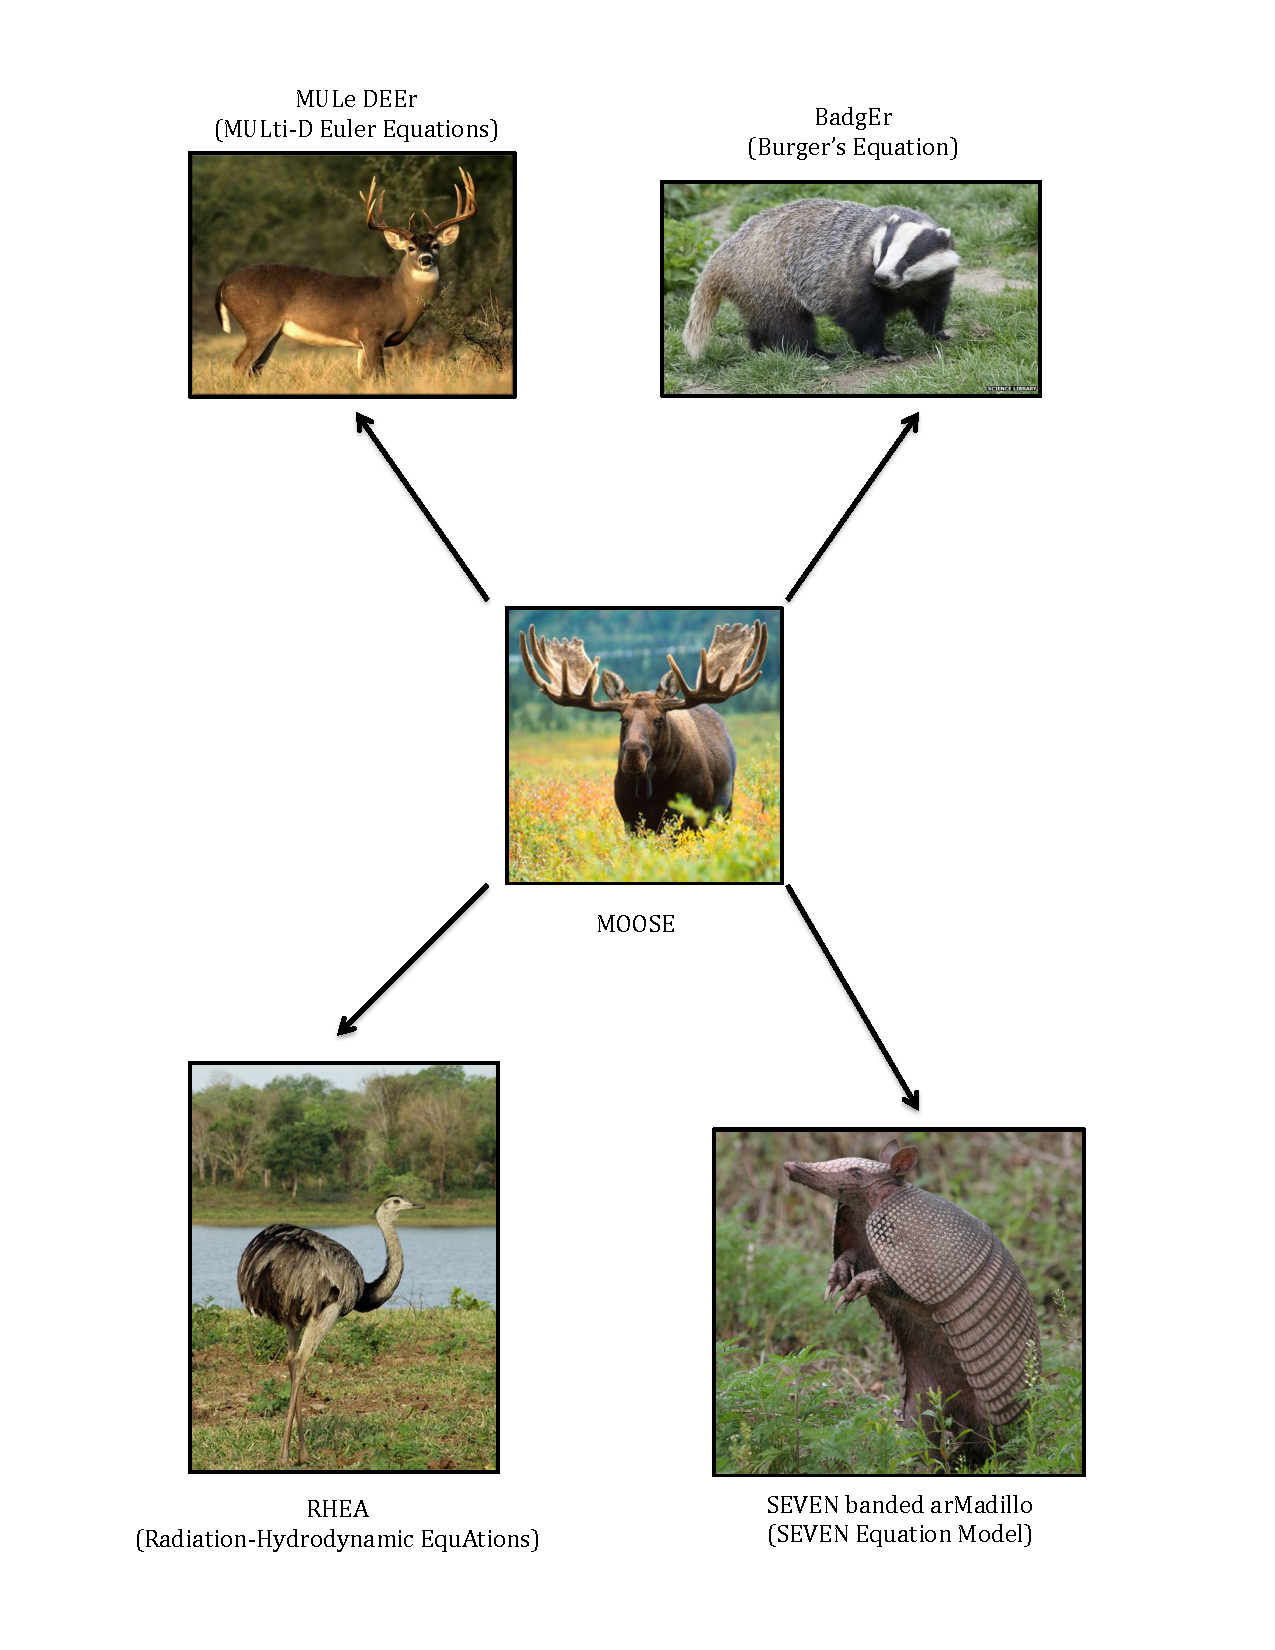
\includegraphics[width=\textwidth]{figures/organigram.pdf}
\caption{Marco's zoo (this is not a food chain). \label{fig:organigram}}
\end{figure}
%